\section{Экспериментальное исследование масштабируемости подхода}
\label{sec:7_experiments} \index{7_experiments}

\subsection{Цели исследования}\label{sec:purpose}

Целью экспериментального исследования являлась оценка масштабируемости предложенного подхода на основе ЦЛП по времени поиска решения при увеличении размерности входных данных.

\subsection{Классы исходных данных}\label{sec:data_classes}

Для исследования использовались три типа входных графов:
\begin{enumerate}
  \item Случайно сгенерированные графы.
  \item Слоистые графы.
  \item Графы работ алгоритма Гаусса-Жордана.
\end{enumerate}

Рассмотрим отдельно каждый тип графов.

\textbf{Случайные графы работ.}

Случайные графы (рис. \ref{fig:sluch_gr}), в которых каждая вершина может иметь 1 или 2 предков и любое количество потомков.

\begin{figure}[!h]
    \centering
    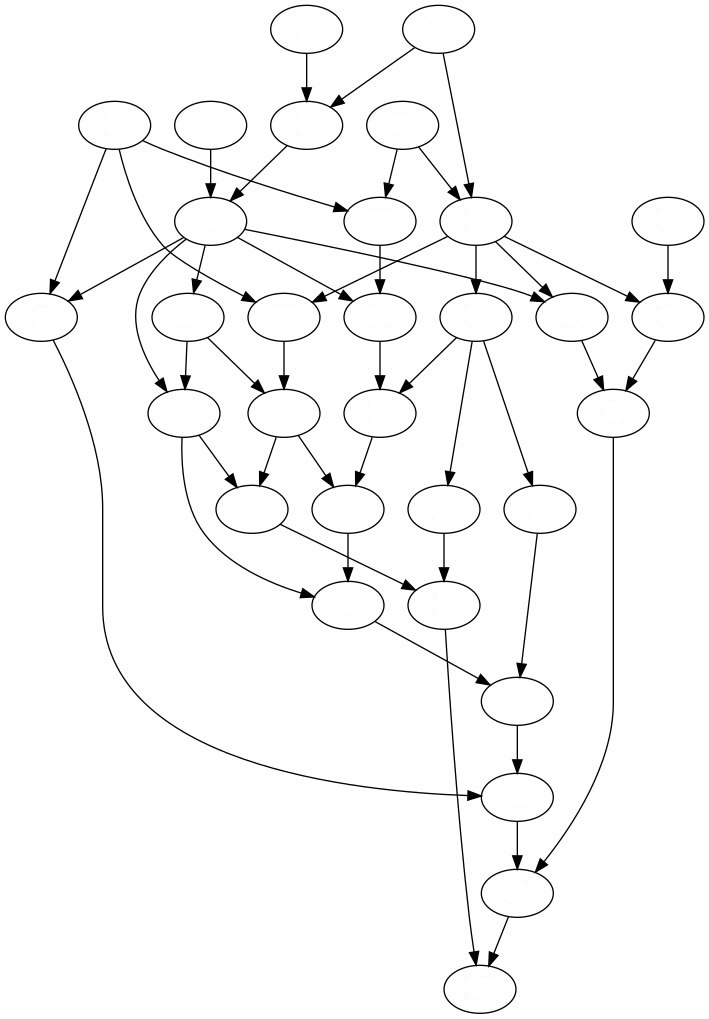
\includegraphics[scale=0.3]{./pictures/схема_случайного_графа.png}
    \caption{Случайный граф.}
    \label{fig:sluch_gr}
\end{figure}


Для экспериментов использовались графы со следующими свойствами:
\begin{itemize}
  \item Количество вершин: от 30 до 97.
  \item Количество ребер: от 41 до 144.
  \item Средняя плотность (количество ребер/количество вершин): 1,47.
  \item Использование ресурсов вершинами: случайное, возможные значения 16384, 65536, 262144.
\end{itemize}

\textbf{Слоистые графы работ.}

Графы работ со слоистой структурой (рис. \ref{fig:sloist_gr}), типичные для многих реальных приложений с многоэтапными вычислениями, например, цифровая обработка сигналов.

\begin{figure}[!h]
    \centering
    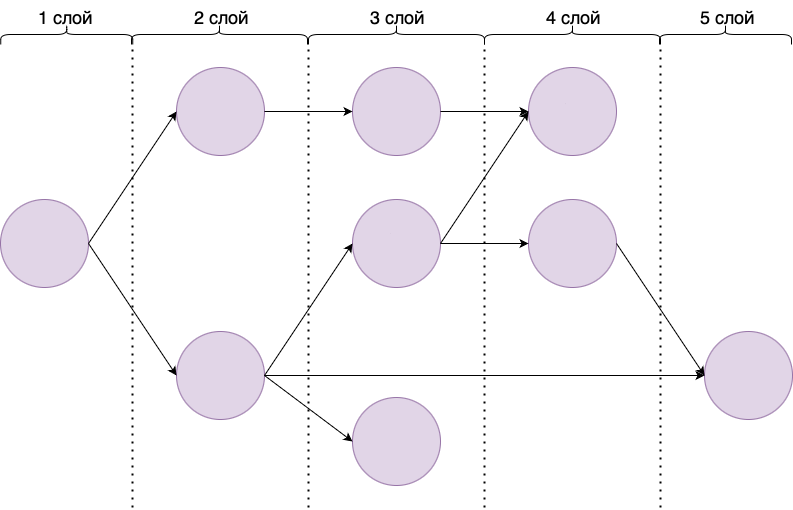
\includegraphics[height=5cm,keepaspectratio]{./pictures/схема_слоистого_графа.png}
    \caption{Слоистый граф.}
    \label{fig:sloist_gr}
\end{figure}

\newpage
Для экспериментов использовались графы со следующими свойствами:
\begin{itemize}
  \item Количество вершин: от 10 до 80 с шагом 5.
  \item Количество ребер: от 9 до 178.
  \item Средняя плотность (количество ребер/количество вершин): 1,49.
  \item Использование ресурсов вершинами: случайное кратное 1024, в диапазоне [2048; 11264].
\end{itemize}

\textbf{Треугольные графы работ.}

Основной набор графов работ для экспериментов по масштабируемости. Этот набор основан на графах работ алгоритма Гаусса-Жордана. Треугольные графы (рис. \ref{fig:treug_graf}) -- это многоуровневые графы с регулярной структурой и ребрами, соединяющими только соседние слои.

\begin{figure}[!h]
    \centering
    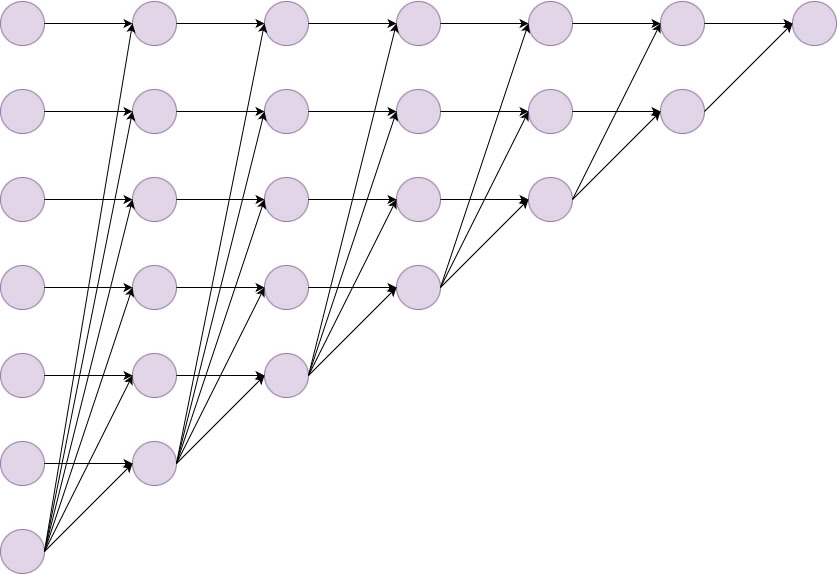
\includegraphics[height=6cm,keepaspectratio]{pictures/схема_треугольного_графа.png}
    \caption{Треугольный граф.}
    \label{fig:treug_graf}
\end{figure}

Для экспериментов использовались графы со следующими свойствами:
\begin{itemize}
  \item Количество вершин: от 21 до 55.
  \item Количество ребер: от 30 до 90.
  \item Средняя плотность (количество ребер/количество вершин): 1,54.
  \item Использование ресурсов вершинами: случайное в диапазоне [1; 100].
\end{itemize}

Количество слоев варьировалось от 6 до 10 с шагом 1. Для каждого количества слоев в наборе есть 6 графов с одинаковой структурой и разным использованием ресурсов вершинами.


\subsection{Результаты экспериментов}
\label{sec:results}

Эксперименты проводились на компьютере со следующими характеристиками:
\begin{itemize}
    \item ЦП: Intel Xeon E5-2650 v4, тактовая частота 2.2 ГГц
    \item Количество ядер: 20
    \item Oбъем ОЗУ: 64 Гб
    \item OС: Ubuntu 20.04 LTS
\end{itemize}

На диаграмме рис. \ref{fig:trianglog} представлено время поиска решения на треугольных графах с использованием решателя SCIP (выбран по результатам предварительных экспериментов, описанных в разделе \ref{sec:4_solvers}). Цвету столбца соответствует наличие или отсутствие транзитивных ребер, а цвету границы столбца -- упорядочение входных данных.

\begin{figure} [h!]
    \centering
    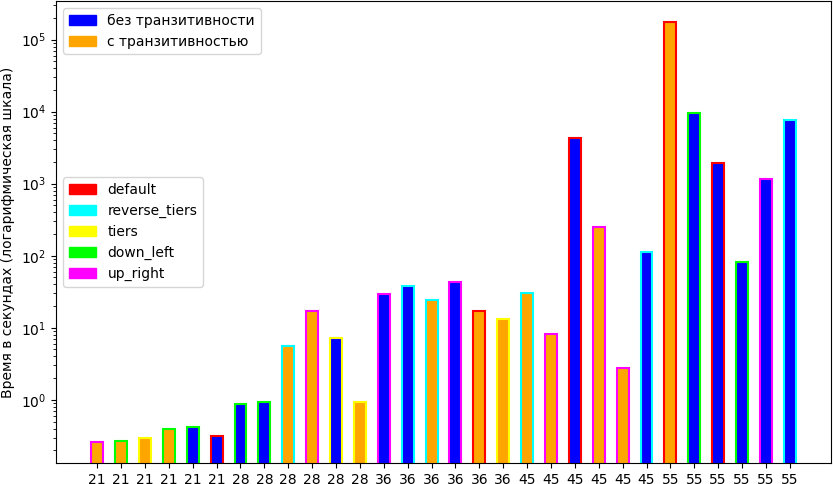
\includegraphics[width=1\linewidth]{pictures/trianglog.png}
    \caption{Время поиска решения на треугольных графах.}
    \label{fig:trianglog}
\end{figure}

Видно, что с ростом числа вершин увеличивается усредненное по графам с одинаковым числом вершин время поиска решения. В зависимости от использования ресурсов вершинами, время поиска при одинаковом числе вершин может различаться в сотни раз (например, для графов с 45 вершинами).

На диаграмме рис. \ref{fig:layeredlog} представлено время поиска решения на слоистых графах. Цвету столбца соответствует наличие или отсутствие транзитивных ребер, а цвету границы столбца -- упорядочение. Под каждым столбцом находится число -- максимальное количество слоев, пропускаемое ребрами, а под этими числами -- число вершин в графе.

\begin{figure}
    \centering
    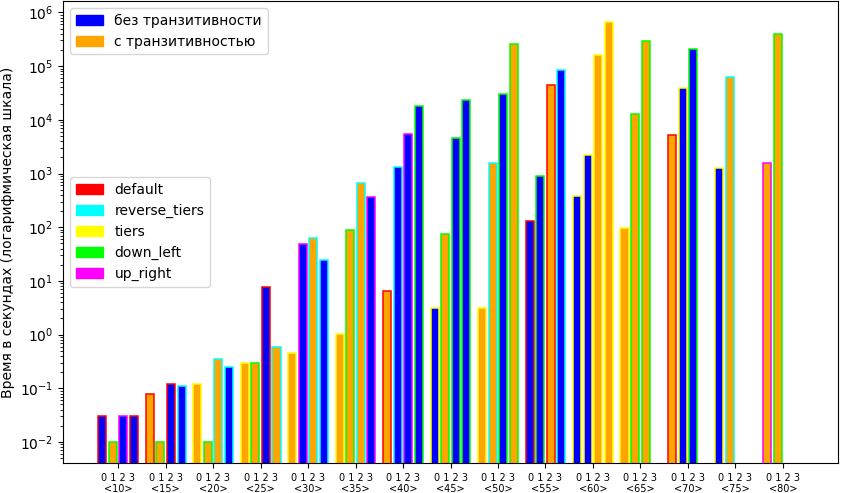
\includegraphics[width=1\linewidth]{pictures/layeredlog.png}
    \caption{Время поиска решения на слоистых графах.}
    \label{fig:layeredlog}
\end{figure}

Видно, что с ростом числа вершин увеличивается усредненное по графам с одинаковым числом вершин время поиска решения. Для фиксированного числа вершин, с увеличением количества пропускаемых слоев время поиска решения растет, порой в десятки раз (например, для графов с 50 вершинами). 

Для случайных графов были построены круговые диаграммы, см. рис. \ref{fig:dagpie}. В легенде каждой диаграммы указано соответствие цвета количеству секунд, понадобившемуся на поиск решения. Ограничение на время работы решателя (TIMELIMIT) было установлено в 3600 секунд.

\newpage
По диаграммам видно, что:
\begin{itemize}
    \item В диапазоне от 30 до 55 вершин около 70\% запусков решателя выполняются менее 100 секунд.
    \item В диапазоне от 55 до 80 вершин большинство запусков решателя выполняются больше 1000 секунд, из них около трети превышают лимит времени.
    \item В диапазоне от 80 до 100 вершин превысили лимит времени 90 процентов запусков решателя, и ни один не  завершился в пределах 1000 секунд.
\end{itemize}

Таким образом, для случайных графов с ростом числа вершин увеличивается минимальное и среднее время нахождения решения, а также растет доля запусков решателя, превысивших ограничение по времени.

\begin{figure}
    \centering
    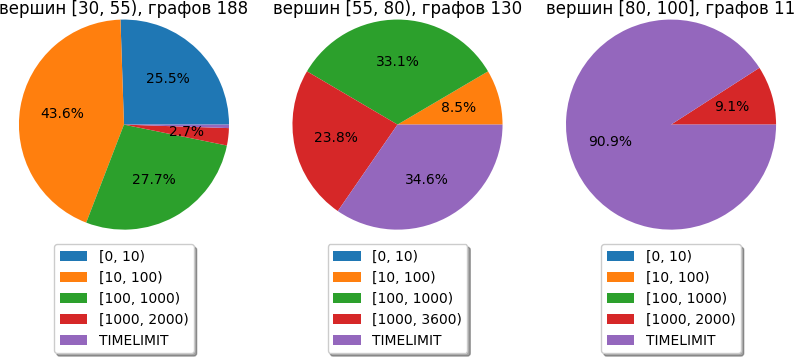
\includegraphics[width=1\linewidth]{pictures/dagpie.png}
    \caption{Время поиска решения на случайных графах.}
    \label{fig:dagpie}
\end{figure}


\subsection{Экономия времени за счет поиска неоптимальных решений}\label{sec:gap}

Решатель SCIP во время поиска оптимального решения находит допустимые, но не оптимальные решения и показывает, насколько лучшее из них отличается по значению целевой функции от оценки оптимума целевой функции, исходя из текущих результатов алгоритма. Формула подсчета отклонения выглядит так:
\[gap = \frac{|primalbound - dualbound|}{min(|primalbound|,|dualbound|)|} * 100\%,\]
где $primalbound$ --- это верхняя оценка оптимального значения, которая равна значению целевой функции лучшего найденного решения задачи, $dualbound$ --- нижняя оценка оптимального значения целевой функции, и знаки $primalbound$ и $dualbound$ совпадают. Если знаки $primalbound$ и $dualbound$ разные, то отклонение ($gap$) принимает значение «Infinity» (бесконечность).

\begin{figure}[h!]
    \centering
    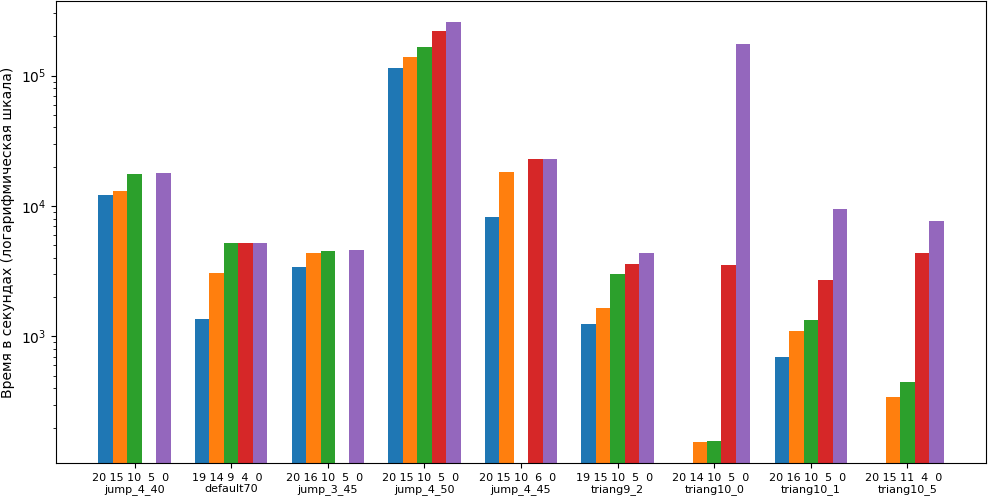
\includegraphics[width=1\linewidth]{template-cmc/pictures/percents_gap.png}
    \caption{Отклонение от теоретической оценки точного решения в процентах.}
    \label{fig:percents_gap}
\end{figure}

По рис. \ref{fig:percents_gap} можно для нескольких графов проследить время поиска решений с верхними оценками отклонения от оптимума в диапазоне от 20\% до 0\% (оптимальное решение) с шагом 5\%. Под столбцами подписаны проценты отклонения, а ниже -- названия графов. Если нужный процент (например, 15\% для графа default70) отсутствовал в протоколе работы решателя, то брался процент на 1 меньше или больше. Если и он отсутствовал, то этот столбец пропускался (например, 5\% для графа jump\_4\_40).

Видно, что в ряде случаев можно значительно сэкономить время, задав небольшое отклонение искомого решения от оптимального по значению целевой функции. Так, для треугольного графа triang10\_0 решение с 10\% отклонением от оптимума ищется более чем в 100 раз быстрее, чем оптимальное решение. В других случаях экономия может быть несущественной, например для слоистого графа jump\_3\_45.




\subsection{Выводы}\label{sec:summary}

Экспериментальное исследование показало быстрый рост времени работы решателя с увеличением размера входного графа, что характерно для NP-трудных задач. При одинаковом количестве вершин в графе, существенное влияние на время работы решателя оказывает как количество потребляемого работами ресурса (видно на треугольных графах), так и структура графа (видно на слоистых графах с различным количеством пропускаемых ребрами слоев).

Выявлена значительная зависимость времени поиска решения от упорядочения входных данных и от наличия или отсутствия добавленных в граф транзитивных ребер. Зависимость не носит систематического характера, поэтому рекомендуется использовать схему с параллельным запуском экземпляров решателя для различных сочетаний упорядочения и наличия/отсутствия транзитивных ребер при одном и том же наборе входных данных задачи.

Ограничения применимости метода по размеру входного графа зависят от структуры графа. В проведенных экспериментах, для треугольных графов максимальное число вершин графа, для которого было найдено решение, составляло 55; для слоистых -- 80 (при отсутствии ребер, пропускающих слои). При этом для треугольного графа с 55 вершинами и 90 ребрами поиск решения занял двое суток, а для слоистого графа с 75 вершинами и 161 ребрами (включая ребра, пропускающие слои) решение не было найдено за 20 суток. Отметим, что в области цифровой обработки сигналов присутствуют графы работ с количеством вершин, не превышающим выявленные пределы: в статье \cite{CASANOVA} приведены графы работ для операций LU-разложения (55 вершин), QR-разложения (55 вершин), разложения Холецкого (35 вершин).

В ряде случаев время работы решателя можно значительно (в десятки раз, до 100 раз) сократить, если остановить поиск при обнаружении решения, отклоняющегося на 10-15\% от оптимального по значению целевой функции.
